% Options for packages loaded elsewhere
% Options for packages loaded elsewhere
\PassOptionsToPackage{unicode}{hyperref}
\PassOptionsToPackage{hyphens}{url}
\PassOptionsToPackage{dvipsnames,svgnames,x11names}{xcolor}
%
\documentclass[
  11pt,
]{article}
\usepackage{xcolor}
\usepackage[margin=2.5cm]{geometry}
\usepackage{amsmath,amssymb}
\setcounter{secnumdepth}{5}
\usepackage{iftex}
\ifPDFTeX
  \usepackage[T1]{fontenc}
  \usepackage[utf8]{inputenc}
  \usepackage{textcomp} % provide euro and other symbols
\else % if luatex or xetex
  \usepackage{unicode-math} % this also loads fontspec
  \defaultfontfeatures{Scale=MatchLowercase}
  \defaultfontfeatures[\rmfamily]{Ligatures=TeX,Scale=1}
\fi
\usepackage{lmodern}
\ifPDFTeX\else
  % xetex/luatex font selection
\fi
% Use upquote if available, for straight quotes in verbatim environments
\IfFileExists{upquote.sty}{\usepackage{upquote}}{}
\IfFileExists{microtype.sty}{% use microtype if available
  \usepackage[]{microtype}
  \UseMicrotypeSet[protrusion]{basicmath} % disable protrusion for tt fonts
}{}
\usepackage{setspace}
\makeatletter
\@ifundefined{KOMAClassName}{% if non-KOMA class
  \IfFileExists{parskip.sty}{%
    \usepackage{parskip}
  }{% else
    \setlength{\parindent}{0pt}
    \setlength{\parskip}{6pt plus 2pt minus 1pt}}
}{% if KOMA class
  \KOMAoptions{parskip=half}}
\makeatother
% Make \paragraph and \subparagraph free-standing
\makeatletter
\ifx\paragraph\undefined\else
  \let\oldparagraph\paragraph
  \renewcommand{\paragraph}{
    \@ifstar
      \xxxParagraphStar
      \xxxParagraphNoStar
  }
  \newcommand{\xxxParagraphStar}[1]{\oldparagraph*{#1}\mbox{}}
  \newcommand{\xxxParagraphNoStar}[1]{\oldparagraph{#1}\mbox{}}
\fi
\ifx\subparagraph\undefined\else
  \let\oldsubparagraph\subparagraph
  \renewcommand{\subparagraph}{
    \@ifstar
      \xxxSubParagraphStar
      \xxxSubParagraphNoStar
  }
  \newcommand{\xxxSubParagraphStar}[1]{\oldsubparagraph*{#1}\mbox{}}
  \newcommand{\xxxSubParagraphNoStar}[1]{\oldsubparagraph{#1}\mbox{}}
\fi
\makeatother

\usepackage{color}
\usepackage{fancyvrb}
\newcommand{\VerbBar}{|}
\newcommand{\VERB}{\Verb[commandchars=\\\{\}]}
\DefineVerbatimEnvironment{Highlighting}{Verbatim}{commandchars=\\\{\}}
% Add ',fontsize=\small' for more characters per line
\usepackage{framed}
\definecolor{shadecolor}{RGB}{241,243,245}
\newenvironment{Shaded}{\begin{snugshade}}{\end{snugshade}}
\newcommand{\AlertTok}[1]{\textcolor[rgb]{0.68,0.00,0.00}{#1}}
\newcommand{\AnnotationTok}[1]{\textcolor[rgb]{0.37,0.37,0.37}{#1}}
\newcommand{\AttributeTok}[1]{\textcolor[rgb]{0.40,0.45,0.13}{#1}}
\newcommand{\BaseNTok}[1]{\textcolor[rgb]{0.68,0.00,0.00}{#1}}
\newcommand{\BuiltInTok}[1]{\textcolor[rgb]{0.00,0.23,0.31}{#1}}
\newcommand{\CharTok}[1]{\textcolor[rgb]{0.13,0.47,0.30}{#1}}
\newcommand{\CommentTok}[1]{\textcolor[rgb]{0.37,0.37,0.37}{#1}}
\newcommand{\CommentVarTok}[1]{\textcolor[rgb]{0.37,0.37,0.37}{\textit{#1}}}
\newcommand{\ConstantTok}[1]{\textcolor[rgb]{0.56,0.35,0.01}{#1}}
\newcommand{\ControlFlowTok}[1]{\textcolor[rgb]{0.00,0.23,0.31}{\textbf{#1}}}
\newcommand{\DataTypeTok}[1]{\textcolor[rgb]{0.68,0.00,0.00}{#1}}
\newcommand{\DecValTok}[1]{\textcolor[rgb]{0.68,0.00,0.00}{#1}}
\newcommand{\DocumentationTok}[1]{\textcolor[rgb]{0.37,0.37,0.37}{\textit{#1}}}
\newcommand{\ErrorTok}[1]{\textcolor[rgb]{0.68,0.00,0.00}{#1}}
\newcommand{\ExtensionTok}[1]{\textcolor[rgb]{0.00,0.23,0.31}{#1}}
\newcommand{\FloatTok}[1]{\textcolor[rgb]{0.68,0.00,0.00}{#1}}
\newcommand{\FunctionTok}[1]{\textcolor[rgb]{0.28,0.35,0.67}{#1}}
\newcommand{\ImportTok}[1]{\textcolor[rgb]{0.00,0.46,0.62}{#1}}
\newcommand{\InformationTok}[1]{\textcolor[rgb]{0.37,0.37,0.37}{#1}}
\newcommand{\KeywordTok}[1]{\textcolor[rgb]{0.00,0.23,0.31}{\textbf{#1}}}
\newcommand{\NormalTok}[1]{\textcolor[rgb]{0.00,0.23,0.31}{#1}}
\newcommand{\OperatorTok}[1]{\textcolor[rgb]{0.37,0.37,0.37}{#1}}
\newcommand{\OtherTok}[1]{\textcolor[rgb]{0.00,0.23,0.31}{#1}}
\newcommand{\PreprocessorTok}[1]{\textcolor[rgb]{0.68,0.00,0.00}{#1}}
\newcommand{\RegionMarkerTok}[1]{\textcolor[rgb]{0.00,0.23,0.31}{#1}}
\newcommand{\SpecialCharTok}[1]{\textcolor[rgb]{0.37,0.37,0.37}{#1}}
\newcommand{\SpecialStringTok}[1]{\textcolor[rgb]{0.13,0.47,0.30}{#1}}
\newcommand{\StringTok}[1]{\textcolor[rgb]{0.13,0.47,0.30}{#1}}
\newcommand{\VariableTok}[1]{\textcolor[rgb]{0.07,0.07,0.07}{#1}}
\newcommand{\VerbatimStringTok}[1]{\textcolor[rgb]{0.13,0.47,0.30}{#1}}
\newcommand{\WarningTok}[1]{\textcolor[rgb]{0.37,0.37,0.37}{\textit{#1}}}

\usepackage{longtable,booktabs,array}
\usepackage{calc} % for calculating minipage widths
% Correct order of tables after \paragraph or \subparagraph
\usepackage{etoolbox}
\makeatletter
\patchcmd\longtable{\par}{\if@noskipsec\mbox{}\fi\par}{}{}
\makeatother
% Allow footnotes in longtable head/foot
\IfFileExists{footnotehyper.sty}{\usepackage{footnotehyper}}{\usepackage{footnote}}
\makesavenoteenv{longtable}
\usepackage{graphicx}
\makeatletter
\newsavebox\pandoc@box
\newcommand*\pandocbounded[1]{% scales image to fit in text height/width
  \sbox\pandoc@box{#1}%
  \Gscale@div\@tempa{\textheight}{\dimexpr\ht\pandoc@box+\dp\pandoc@box\relax}%
  \Gscale@div\@tempb{\linewidth}{\wd\pandoc@box}%
  \ifdim\@tempb\p@<\@tempa\p@\let\@tempa\@tempb\fi% select the smaller of both
  \ifdim\@tempa\p@<\p@\scalebox{\@tempa}{\usebox\pandoc@box}%
  \else\usebox{\pandoc@box}%
  \fi%
}
% Set default figure placement to htbp
\def\fps@figure{htbp}
\makeatother





\setlength{\emergencystretch}{3em} % prevent overfull lines

\providecommand{\tightlist}{%
  \setlength{\itemsep}{0pt}\setlength{\parskip}{0pt}}



 


\makeatletter
\@ifpackageloaded{caption}{}{\usepackage{caption}}
\AtBeginDocument{%
\ifdefined\contentsname
  \renewcommand*\contentsname{Table of contents}
\else
  \newcommand\contentsname{Table of contents}
\fi
\ifdefined\listfigurename
  \renewcommand*\listfigurename{List of Figures}
\else
  \newcommand\listfigurename{List of Figures}
\fi
\ifdefined\listtablename
  \renewcommand*\listtablename{List of Tables}
\else
  \newcommand\listtablename{List of Tables}
\fi
\ifdefined\figurename
  \renewcommand*\figurename{Figure}
\else
  \newcommand\figurename{Figure}
\fi
\ifdefined\tablename
  \renewcommand*\tablename{Table}
\else
  \newcommand\tablename{Table}
\fi
}
\@ifpackageloaded{float}{}{\usepackage{float}}
\floatstyle{ruled}
\@ifundefined{c@chapter}{\newfloat{codelisting}{h}{lop}}{\newfloat{codelisting}{h}{lop}[chapter]}
\floatname{codelisting}{Listing}
\newcommand*\listoflistings{\listof{codelisting}{List of Listings}}
\makeatother
\makeatletter
\makeatother
\makeatletter
\@ifpackageloaded{caption}{}{\usepackage{caption}}
\@ifpackageloaded{subcaption}{}{\usepackage{subcaption}}
\makeatother
\usepackage{bookmark}
\IfFileExists{xurl.sty}{\usepackage{xurl}}{} % add URL line breaks if available
\urlstyle{same}
\hypersetup{
  pdftitle={Replica curva del tasso di inflazione secondo BCE},
  pdfauthor={Paolo Volterra},
  pdfkeywords={BCE, inflazione, qmd},
  colorlinks=true,
  linkcolor={blue},
  filecolor={Maroon},
  citecolor={Blue},
  urlcolor={Blue},
  pdfcreator={LaTeX via pandoc}}


\title{Replica curva del tasso di inflazione secondo BCE}
\usepackage{etoolbox}
\makeatletter
\providecommand{\subtitle}[1]{% add subtitle to \maketitle
  \apptocmd{\@title}{\par {\large #1 \par}}{}{}
}
\makeatother
\subtitle{Studio sui dati BCE}
\author{Paolo Volterra}
\date{}
\begin{document}
\maketitle

\renewcommand*\contentsname{Table of contents}
{
\hypersetup{linkcolor=}
\setcounter{tocdepth}{3}
\tableofcontents
}

\setstretch{1.3}
\section{Tassi di inflazione trimestrali
YoY}\label{tassi-di-inflazione-trimestrali-yoy}

\begin{itemize}
\tightlist
\item
  Proviamo a replicare questo grafico preso da
  \href{https://www.allianz-trade.com/content/dam/onemarketing/aztrade/allianz-trade_com/it_it/allianz-trade-it/news-e-approfondimenti/pdf-studi-economici/mid-year-economic-outlook-2025-26.pdf}{Allianz.
  (2025). \_Mid-year Economic Outlook 2025-26}
\item
  Il file pdf è in \href{zotero://select/library/items/FD23KCPH}{Zotero}
\item
  Per BCE, questa è la series key: \textbf{ICP.M.U2.N.000000.4.ANR}
  \href{https://data.ecb.europa.eu/data/datasets/ICP/ICP.M.U2.N.000000.4.ANR}{HICP
  - Overall index, Euro area (changing composition), Monthly}
\end{itemize}

\pandocbounded{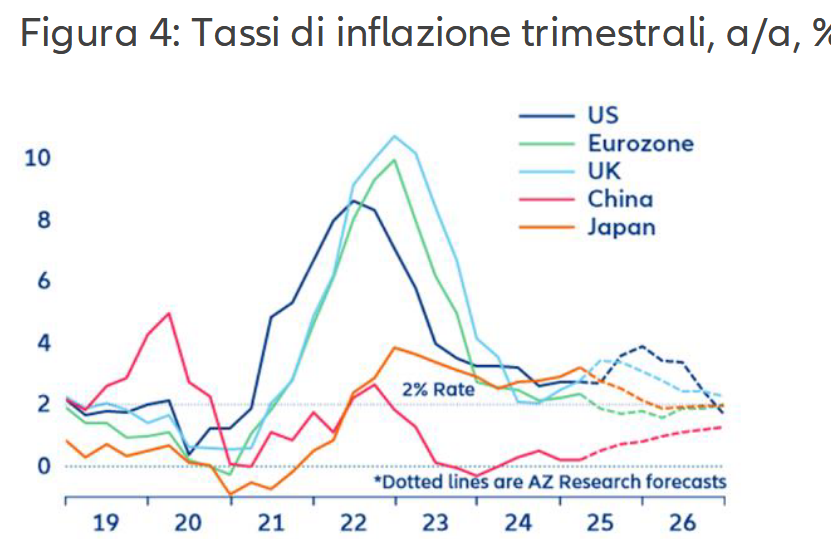
\includegraphics[keepaspectratio]{./media/Pasted image 20250726085321.png}}

\begin{Shaded}
\begin{Highlighting}[]
\ImportTok{from}\NormalTok{ ecbdata }\ImportTok{import}\NormalTok{ ecbdata}
\ImportTok{import}\NormalTok{ pandas }\ImportTok{as}\NormalTok{ pd}
\ImportTok{import}\NormalTok{ matplotlib.pyplot }\ImportTok{as}\NormalTok{ plt}
\ImportTok{from}\NormalTok{ matplotlib }\ImportTok{import}\NormalTok{ rcParams}

\CommentTok{\# https://data.ecb.europa.eu/data/datasets/EXR/EXR.M.USD.EUR.SP00.A}
\NormalTok{df }\OperatorTok{=}\NormalTok{ ecbdata.get\_series(}\StringTok{\textquotesingle{}ICP.M.U2.N.000000.4.ANR\textquotesingle{}}\NormalTok{ , start}\OperatorTok{=}\StringTok{\textquotesingle{}2019{-}01\textquotesingle{}}\NormalTok{) }\CommentTok{\#}
\NormalTok{df.TIME\_PERIOD }\OperatorTok{=}\NormalTok{ pd.to\_datetime(df.TIME\_PERIOD)}
\NormalTok{df }\OperatorTok{=}\NormalTok{ df.set\_index(}\StringTok{\textquotesingle{}TIME\_PERIOD\textquotesingle{}}\NormalTok{)}
\end{Highlighting}
\end{Shaded}

\begin{Shaded}
\begin{Highlighting}[]
\ImportTok{import}\NormalTok{ matplotlib.pyplot }\ImportTok{as}\NormalTok{ plt}
\ImportTok{import}\NormalTok{ pandas }\ImportTok{as}\NormalTok{ pd}
\ImportTok{from}\NormalTok{ matplotlib }\ImportTok{import}\NormalTok{ rcParams}

\CommentTok{\# Aggiorna configurazione dei font per aumentare dimensioni}
\NormalTok{rcParams.update(\{}
    \StringTok{\textquotesingle{}font.family\textquotesingle{}}\NormalTok{: }\StringTok{\textquotesingle{}serif\textquotesingle{}}\NormalTok{,}
    \StringTok{\textquotesingle{}font.serif\textquotesingle{}}\NormalTok{: [}\StringTok{\textquotesingle{}Georgia\textquotesingle{}}\NormalTok{, }\StringTok{\textquotesingle{}Times New Roman\textquotesingle{}}\NormalTok{, }\StringTok{\textquotesingle{}serif\textquotesingle{}}\NormalTok{],}
    \StringTok{\textquotesingle{}axes.titlesize\textquotesingle{}}\NormalTok{: }\DecValTok{16}\NormalTok{,}
    \StringTok{\textquotesingle{}axes.labelsize\textquotesingle{}}\NormalTok{: }\DecValTok{14}\NormalTok{,}
    \StringTok{\textquotesingle{}xtick.labelsize\textquotesingle{}}\NormalTok{: }\DecValTok{12}\NormalTok{,}
    \StringTok{\textquotesingle{}ytick.labelsize\textquotesingle{}}\NormalTok{: }\DecValTok{12}\NormalTok{,}
    \StringTok{\textquotesingle{}legend.fontsize\textquotesingle{}}\NormalTok{: }\DecValTok{12}\NormalTok{,}
\NormalTok{\})}

\CommentTok{\# Imposta larghezza e altezza in pollici}
\NormalTok{fig, ax }\OperatorTok{=}\NormalTok{ plt.subplots(figsize}\OperatorTok{=}\NormalTok{(}\DecValTok{10}\NormalTok{, }\DecValTok{6}\NormalTok{))}

\CommentTok{\# Linea principale}
\NormalTok{df.OBS\_VALUE.plot(ax}\OperatorTok{=}\NormalTok{ax, color}\OperatorTok{=}\StringTok{\textquotesingle{}\#007a53\textquotesingle{}}\NormalTok{, linewidth}\OperatorTok{=}\DecValTok{3}\NormalTok{)}

\CommentTok{\# Titolo e asse Y}
\NormalTok{plt.title(}\StringTok{"Inflazione Armonizzata (HICP) {-} Eurozona"}\NormalTok{)}
\NormalTok{plt.ylabel(}\StringTok{"\% YoY"}\NormalTok{)}

\CommentTok{\# Asse X}
\NormalTok{ax.set\_xticks(pd.date\_range(}\StringTok{"2019{-}01{-}01"}\NormalTok{, }\StringTok{"2026{-}01{-}01"}\NormalTok{, freq}\OperatorTok{=}\StringTok{"YS"}\NormalTok{))}
\NormalTok{ax.set\_xticklabels([}\BuiltInTok{str}\NormalTok{(y)[}\DecValTok{2}\NormalTok{:] }\ControlFlowTok{for}\NormalTok{ y }\KeywordTok{in} \BuiltInTok{range}\NormalTok{(}\DecValTok{2019}\NormalTok{, }\DecValTok{2027}\NormalTok{)])}

\CommentTok{\# Asse Y con estensione negativa}
\NormalTok{ax.set\_ylim(}\OperatorTok{{-}}\DecValTok{1}\NormalTok{, }\DecValTok{11}\NormalTok{)}
\NormalTok{ax.set\_yticks(}\BuiltInTok{range}\NormalTok{(}\DecValTok{0}\NormalTok{, }\DecValTok{12}\NormalTok{, }\DecValTok{2}\NormalTok{))}

\CommentTok{\# Griglia e bordi}
\NormalTok{ax.grid(}\VariableTok{False}\NormalTok{)}
\NormalTok{ax.spines[}\StringTok{\textquotesingle{}top\textquotesingle{}}\NormalTok{].set\_visible(}\VariableTok{False}\NormalTok{)}
\NormalTok{ax.spines[}\StringTok{\textquotesingle{}right\textquotesingle{}}\NormalTok{].set\_visible(}\VariableTok{False}\NormalTok{)}

\CommentTok{\# Linea del 2\%}
\NormalTok{ax.axhline(}\DecValTok{2}\NormalTok{, color}\OperatorTok{=}\StringTok{\textquotesingle{}gray\textquotesingle{}}\NormalTok{, linestyle}\OperatorTok{=}\StringTok{\textquotesingle{}{-}{-}\textquotesingle{}}\NormalTok{, linewidth}\OperatorTok{=}\FloatTok{0.8}\NormalTok{)}
\NormalTok{ax.text(df.index[}\DecValTok{6}\NormalTok{], }\FloatTok{2.2}\NormalTok{, }\StringTok{"2\% Rate"}\NormalTok{, fontsize}\OperatorTok{=}\DecValTok{12}\NormalTok{, color}\OperatorTok{=}\StringTok{"gray"}\NormalTok{)}

\CommentTok{\# Layout finale}
\NormalTok{plt.tight\_layout()}
\NormalTok{plt.show()}
\end{Highlighting}
\end{Shaded}

\pandocbounded{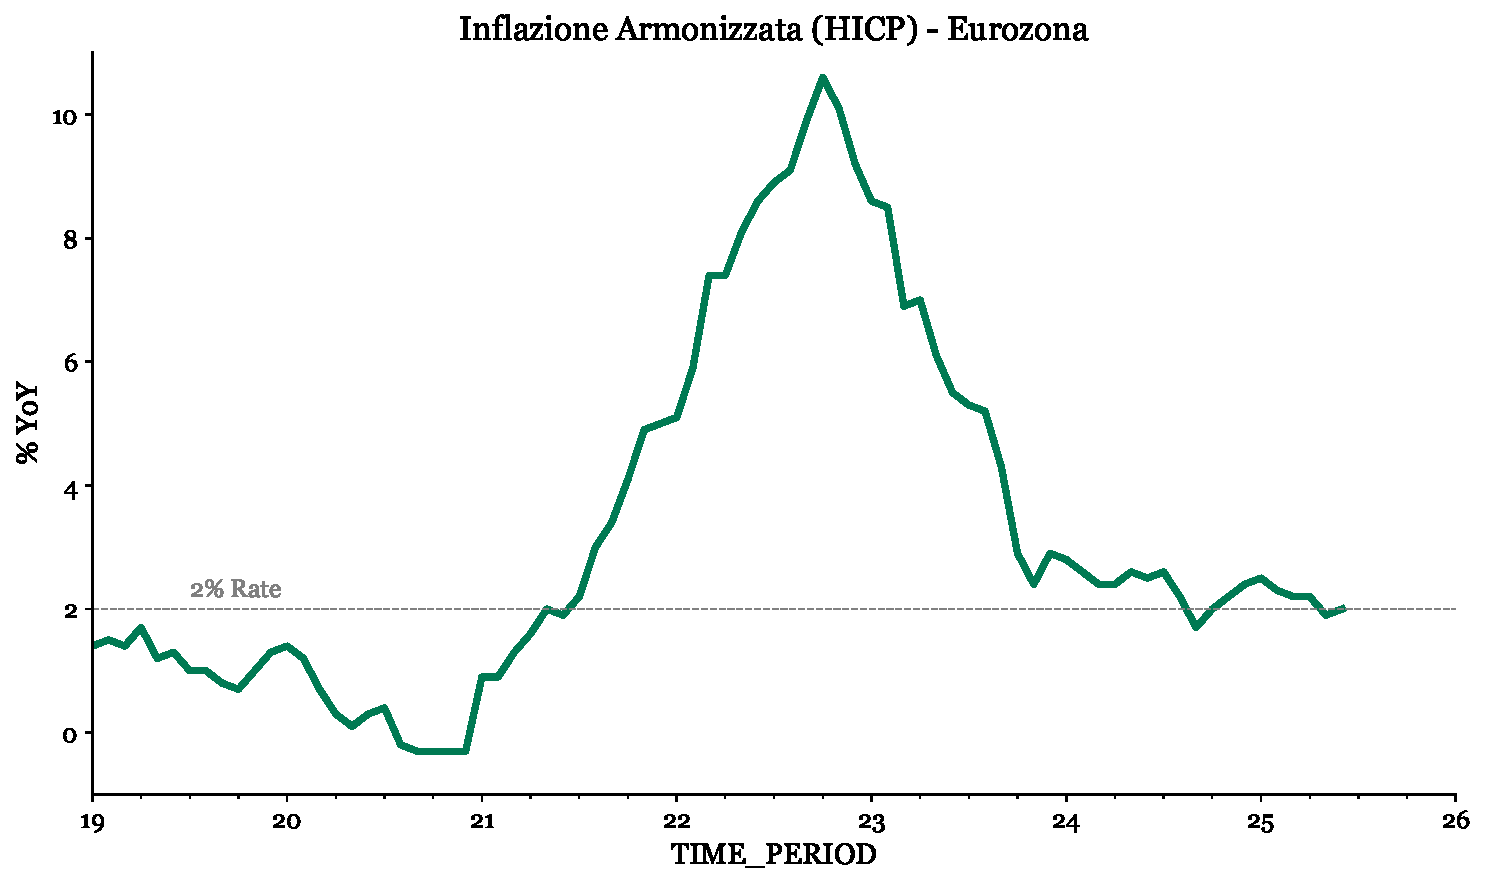
\includegraphics[keepaspectratio]{2025072502_BCE_inflazione_files/figure-pdf/cell-3-output-1.pdf}}




\end{document}
